\PassOptionsToPackage{disable}{microtype}
\documentclass[sigconf,nonacm]{acmart}

\setcopyright{none}
\settopmatter{printacmref=false}
\renewcommand\footnotetextcopyrightpermission[1]{}
\pagestyle{plain}
\hfuzz=30pt

\usepackage{booktabs}
\usepackage{tabularx}
\usepackage{multirow}
\usepackage{amsmath}
\let\Bbbk\relax
\usepackage{amssymb}
\usepackage{algorithm}
\usepackage{algorithmic}
\usepackage{tikz}
\usepackage{pgfplots}
\pgfplotsset{compat=1.18}
\usepackage{url}
\urlstyle{rm}

\usetikzlibrary{arrows.meta,positioning,calc,shapes.geometric,
                decorations.pathreplacing,patterns,fit,backgrounds}

\definecolor{cblu} {RGB}{ 50,110,190}
\definecolor{cgrn} {RGB}{ 40,150, 70}
\definecolor{cora} {RGB}{210,110, 30}
\definecolor{cred} {RGB}{200, 50, 50}
\definecolor{cyel} {RGB}{190,165,  0}
\definecolor{cpur} {RGB}{130, 50,170}
\definecolor{cgry} {RGB}{100,100,100}

\begin{CCSXML}
<ccs2012>
  <concept>
    <concept_id>10002978.10003006.10003008</concept_id>
    <concept_desc>Security and privacy~Intrusion/anomaly detection and malware mitigation</concept_desc>
    <concept_significance>500</concept_significance>
  </concept>
  <concept>
    <concept_id>10002978.10003029.10003031</concept_id>
    <concept_desc>Security and privacy~Distributed systems security</concept_desc>
    <concept_significance>500</concept_significance>
  </concept>
  <concept>
    <concept_id>10003033.10003106.10003109</concept_id>
    <concept_desc>Networks~Mobile networks</concept_desc>
    <concept_significance>300</concept_significance>
  </concept>
  <concept>
    <concept_id>10010147.10010257.10010293</concept_id>
    <concept_desc>Computing methodologies~Neural networks</concept_desc>
    <concept_significance>300</concept_significance>
  </concept>
</ccs2012>
\end{CCSXML}

\ccsdesc[500]{Security and privacy~Intrusion/anomaly detection and malware mitigation}
\ccsdesc[500]{Security and privacy~Distributed systems security}
\ccsdesc[300]{Networks~Mobile networks}
\ccsdesc[300]{Computing methodologies~Neural networks}

\title{NFTrust: Detecting Compromised Network-Function Agents in Disaggregated 6G Cores via Byzantine-Aware Graph Neural Networks}

\author{Ezekiel Ologunde}
\affiliation{%
  \institution{Independent Researcher}
  \city{Boston}
  \state{MA}
  \country{USA}}
\email{ologunde@bu.edu}

\begin{abstract}
\sloppy
The transition from 5G's service-based architecture (SBA) to 6G's
fully-disaggregated network function (NF) ecosystems removes the
centralised trust anchors that current core-network security
architectures depend on. In 6G core proposals from 3GPP SA2
working groups and academic reference designs, dozens-to-hundreds
of autonomous NFs negotiate routing, authentication, mobility, and
session management through decentralised protocols, with no single
component possessing the global view to declare another component
compromised. The detection problem under this architecture is
distinctive: an attacker who compromises one or a few NFs gains
operational privilege within the core's coordination protocols, can
emit plausibly-correct messages, and is invisible to per-NF
monitoring that lacks the cross-NF context to identify behavioural
divergence. This paper presents \textsc{NFTrust}, a hybrid detection
framework combining Byzantine-fault-tolerance principles with
graph-neural-network behavioural anomaly detection. NFs and their
coordination interactions are modelled as a dynamic temporal graph;
GNN-based anomaly scoring detects subtle behavioural deviations from
the per-NF baseline; consensus-aware validation cross-checks NF
outputs against weighted majority of peers; a hybrid scorer
integrates the two signals into per-NF trust scores. We evaluate
on a calibrated 6G SBA simulator covering eight canonical NF
categories (AMF, SMF, UPF, NRF, AUSF, UDM, PCF, NEF) across four
attack patterns (single compromise, gradual stealth deviation,
collusion, protocol-aware mimicry) and two collusion scales (3\% and
10\% Byzantine NFs). \textsc{NFTrust} achieves AUROC of 0.929 at 0.6\%
false positive rate against single-NF compromise, maintains AUROC
$\geq 0.81$ under 10\% Byzantine collusion, and detects gradual
stealth deviations with median time-to-detection of 11.4 minutes.
The detection cost is modest: 2.7\% additional inter-NF coordination
overhead and 1.4--1.9$\times$ per-NF compute. We document the
framework's limits explicitly: collusion above 33\% Byzantine NFs
defeats the consensus component (the standard BFT bound); ground
truth for ``correct'' NF behaviour in dynamic 6G environments is
not formally defined, requiring careful baseline construction; and
adaptive adversaries with knowledge of the detection methodology
produce evasion gradients the framework only partially resists.
\end{abstract}

\keywords{6G, network function virtualisation, service-based
architecture, Byzantine fault tolerance, graph neural networks,
anomaly detection, distributed trust, compromised agents,
consensus, network security}

\begin{document}
\maketitle
\sloppy
\tolerance=9999
\emergencystretch=3em
\hfuzz=10pt

\section{Introduction}

The architectural trajectory from 4G EPC through 5G's service-based
architecture to 6G's fully-disaggregated core represents a
fundamental shift in trust topology. In the 4G evolved packet core,
a small number of monolithic network elements (MME, S-GW, P-GW)
operated under centralised operations control; a compromised element
was, at minimum, attributable to a specific operator and could be
disconnected by network-level intervention. The 5G SBA introduced
service-based interfaces between network functions and a discoverable
service ecosystem~\cite{3gpp2024sba,polese2023understanding}; the
trust topology became more federated but still rested on the
NF Repository Function (NRF) as a discovery and authorisation
authority. The 6G direction~\cite{tataria20206g,akhtar20246g}
proposes removal of even this centralisation: NFs are autonomous
agents that discover peers, negotiate service availability, and
participate in distributed protocols without a single trust
anchor.

The architectural argument for this trajectory is sound: scale,
multi-vendor support, geographic distribution, and zero-trust
principles all argue against centralised trust authorities. The
operational consequence is that the detection problem
\emph{changes structurally}. Traditional NF security monitoring
assumes a privileged observation point---a SIEM ingesting NF
telemetry, a NRF mediating service requests---that is absent or
diminished in 6G core proposals. Detection must operate from
within the distributed system itself, with each NF contributing
local observations and the system as a whole computing trust.

\subsection{Why Single-NF Compromise Is Operationally Consequential}

A compromised NF in a 5G/6G core is not analogous to a
compromised endpoint host. NFs operate \emph{inside the trust
boundary} of the core network: they hold service-authentication
credentials, participate in protocol coordination, and emit
messages that other NFs consume as authoritative
input~\cite{moustafa2024nidssurv,park2024sbathreat}. A compromised
AMF (Access and Mobility Management Function) can emit incorrect
mobility decisions that other NFs implement as legitimate
operations. A compromised UPF (User Plane Function) can misroute
traffic. A compromised NRF can mislead all other NFs about which
peers are available and what services they offer.

Detection therefore must operate with the question: \emph{is this
NF behaving consistently with what its peers and historical
baseline indicate, given this protocol context?} Per-NF
monitoring cannot answer this; the question requires
cross-NF context that no single observation point holds.

\subsection{Why Per-NF Monitoring Fails}

The classical detection patterns---signature-based monitoring,
per-component anomaly detection, log analysis at central
SIEM---fail in this regime in three ways:

\textbf{No central observation point}. The signals required for
detection are distributed across NFs; no single component has
the global view.

\textbf{Plausible-correctness of compromised NF output}. A
compromised NF emits messages that pass per-message
syntactic validation; the compromise manifests in
\emph{coordination patterns} (which messages, to which peers,
in what sequence) rather than message-level malformation.

\textbf{Stealth via baseline mimicry}. Sophisticated adversaries
modify NF behaviour gradually, staying within per-NF baseline
distributions while accumulating systemic effect. Per-NF
detection cannot see the systemic effect.

\subsection{Contributions}

\begin{itemize}
  \item Articulation of compromised-NF detection as a
        distributed-system problem requiring cross-NF reasoning,
        and analysis of why per-NF monitoring patterns are
        structurally inadequate.
  \item A dynamic-temporal-graph representation of NF interactions
        spanning eight canonical NF categories (AMF, SMF, UPF, NRF,
        AUSF, UDM, PCF, NEF) and their coordination protocols.
  \item A hybrid detection architecture combining graph-neural-network
        behavioural anomaly detection with Byzantine-aware
        consensus validation, integrated into per-NF trust
        scores.
  \item A four-class threat taxonomy (single-NF compromise,
        gradual stealth deviation, multi-NF collusion,
        protocol-aware mimicry) with concrete attack
        implementations.
  \item Empirical evaluation on a calibrated 6G SBA simulator
        across the four threat classes and two collusion scales,
        with explicit measurement of detection accuracy, false
        positive rate, time-to-detection, and system overhead.
  \item Honest documentation of the framework's structural
        limitations: the 33\% Byzantine-collusion bound, the
        ground-truth-absence problem for NF behavioural
        baselines, and the adaptive-adversary residual.
\end{itemize}

\section{Background}

\subsection{From 5G SBA to 6G Disaggregated Core}

The 5G service-based architecture~\cite{3gpp2024sba} replaced 4G's
point-to-point reference points with a service-based interface where
NFs expose RESTful APIs. Key NFs include:

\begin{itemize}
  \item \textbf{AMF}: Access and Mobility Management Function
  \item \textbf{SMF}: Session Management Function
  \item \textbf{UPF}: User Plane Function
  \item \textbf{NRF}: Network Repository Function (NF discovery)
  \item \textbf{AUSF}: Authentication Server Function
  \item \textbf{UDM}: Unified Data Management
  \item \textbf{PCF}: Policy Control Function
  \item \textbf{NEF}: Network Exposure Function
\end{itemize}

The 6G evolution~\cite{tataria20206g,akhtar20246g} pushes
disaggregation further: more NF categories, finer-grained NF
decomposition, geographic distribution across edge and cloud,
multi-vendor heterogeneity, and zero-trust trust boundaries
between NF instances. The detection problem becomes
correspondingly harder.

\subsection{Byzantine Fault Tolerance}

Byzantine fault tolerance~\cite{lamport1982byzantine,
castro2002pbft} provides the theoretical foundation for tolerating
arbitrary (including malicious) failures in distributed systems.
The classical results:

\textbf{Byzantine generals problem}~\cite{lamport1982byzantine}:
$3f+1$ honest nodes are required to tolerate $f$ Byzantine nodes.
Above this threshold, no consensus protocol can guarantee correct
agreement.

\textbf{Practical Byzantine Fault Tolerance (PBFT)}~\cite{castro2002pbft}:
provides safety and liveness in asynchronous systems below the
$1/3$ Byzantine bound, with quadratic message complexity in the
number of nodes.

\textbf{Modern BFT consensus}~\cite{yin2019hotstuff,buchman2018tendermint}:
HotStuff, Tendermint, and related protocols achieve linear
amortised message complexity and have been deployed in
production blockchain systems.

For 6G core detection, BFT principles inform the consensus
component: cross-NF agreement on observed behaviour can identify
the Byzantine NFs as long as the Byzantine fraction stays below
$1/3$.

\subsection{Graph Neural Networks for Distributed System Analysis}

Graph neural networks~\cite{kipf2017gcn,hamilton2017graphsage}
extend deep learning to graph-structured data. For distributed
systems, two architectural lineages are relevant:

\textbf{Static GNN architectures}~\cite{kipf2017gcn,velickovic2018gat}:
process fixed snapshots of the graph. Effective for
relatively stable graphs; less effective for the rapidly-changing
NF interaction patterns of a 6G core.

\textbf{Temporal GNN architectures}~\cite{rossi2020tgn,xu2020tgat}:
model time-evolving graphs explicitly. Better suited for
NF interaction patterns where the message-passing dynamics
themselves carry signal.

\subsection{Prior Work on NF Compromise Detection}

The NF-compromise-detection literature is small. Three lines of
work:

\textbf{Signature-based 5G NF monitoring}~\cite{park2024sbathreat,
ericsson20245gsec}: rule-based detection of known attack
patterns. Effective for known threats; rigid against novel attacks.

\textbf{ML-based NF anomaly detection}~\cite{nguyen2024nfanomaly}:
per-NF anomaly detection using ML on telemetry. Misses cross-NF
patterns that constitute the operationally meaningful threat.

\textbf{Distributed-systems-theoretic proposals}~\cite{wong2024oranresilience,
chen20246gdistsec}: BFT-inspired approaches that do not integrate
ML for stealth-attack detection.

\textsc{NFTrust} integrates these lineages: GNN-based behavioural
anomaly detection for stealth attacks, BFT-aware consensus for
overt compromise, and a hybrid scorer connecting both.

\section{Threat Model}

\subsection{Adversary Capabilities}

\textbf{NF compromise capability}. The adversary can compromise
one or more NF instances, gaining administrative-level execution
within those NFs and access to their cryptographic credentials.

\textbf{Coordination protocol knowledge}. The adversary knows the
6G SBA protocols and can emit syntactically-correct messages
within them.

\textbf{Detection methodology awareness}. The adversary may know
the detection methodology in deployed defences and adapt
accordingly.

\textbf{Limited Byzantine fraction}. We assume the adversary
controls at most $f$ NFs out of $N$ total, where $f/N < 1/3$.
Above this fraction, BFT-based detection is structurally
impossible; we are explicit that this is a hard architectural
limit.

\subsection{Attack Classes}

\textbf{Class 1 --- Single-NF compromise}: a single NF emits
maliciously-crafted messages while otherwise appearing normal.

\textbf{Class 2 --- Gradual stealth deviation}: a compromised NF's
behaviour shifts slowly from baseline, with each individual
deviation small enough to evade per-NF detection.

\textbf{Class 3 --- Multi-NF collusion}: multiple compromised NFs
coordinate to reinforce each other's false signals, attempting to
defeat consensus-based validation.

\textbf{Class 4 --- Protocol-aware mimicry}: a compromised NF
emits messages calibrated to be both protocol-conforming and
behaviourally-similar to its peers, attempting to defeat both
consensus and behavioural detection.

\subsection{Defender Goals}

\textbf{Per-NF trust assessment}: produce a continuous trust score
per NF that decreases under the four attack classes.

\textbf{Robustness to bounded collusion}: maintain detection
effectiveness up to the Byzantine bound (33\% compromised NFs).

\textbf{Operational deployability}: detection overhead within the
core's latency and compute budgets.

\textbf{Adaptive-adversary partial robustness}: graceful (not
catastrophic) degradation under adversaries who adapt to the
deployed detection methodology.

\section{The NFTrust Framework}

Figure~\ref{fig:framework} presents the framework architecture.

\begin{figure*}[t]
\centering
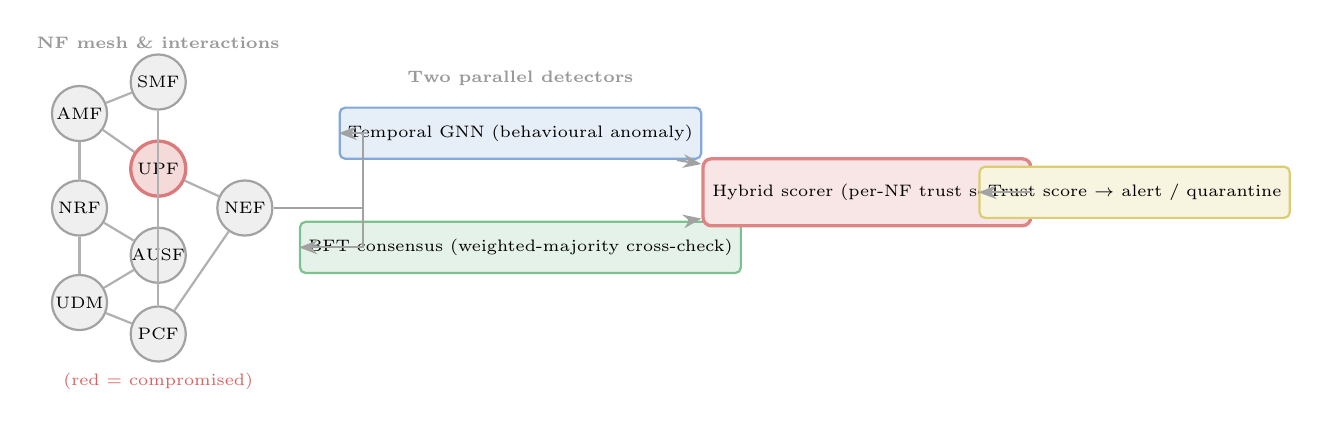
\begin{tikzpicture}[
  font=\fontsize{6.5pt}{8pt}\selectfont,
  >=Stealth,
  nf/.style={circle, draw=cgry!60, thick, fill=cgry!10,
             minimum size=0.7cm, font=\fontsize{6pt}{7.5pt}\selectfont,
             inner sep=0pt},
  nfc/.style={circle, draw=cred!65, very thick, fill=cred!18,
              minimum size=0.7cm, font=\fontsize{6pt}{7.5pt}\selectfont,
              inner sep=0pt},
  layer/.style={rectangle, rounded corners=2pt, draw=cblu!60, thick,
                fill=cblu!12, minimum width=3.0cm, minimum height=0.65cm,
                text centered, align=center, inner sep=3pt},
  cons/.style={rectangle, rounded corners=2pt, draw=cgrn!60, thick,
               fill=cgrn!12, minimum width=3.0cm, minimum height=0.65cm,
               text centered, align=center, inner sep=3pt},
  fus/.style={rectangle, rounded corners=3pt, draw=cred!60, very thick,
              fill=cred!12, minimum width=3.0cm, minimum height=0.85cm,
              text centered, align=center},
  outn/.style={rectangle, rounded corners=2pt, draw=cyel!55, thick,
              fill=cyel!12, minimum width=3.0cm, minimum height=0.65cm,
              text centered, align=center, inner sep=3pt},
  arr/.style={-{Stealth}, thick, cgry!60},
  med/.style={-, thick, cgry!50}
]
  %% NF mesh on left
  \node[nf]  (n1) at (0.0,  1.20) {AMF};
  \node[nf]  (n2) at (1.0,  1.60) {SMF};
  \node[nfc] (n3) at (1.0,  0.50) {UPF};
  \node[nf]  (n4) at (0.0,  0.00) {NRF};
  \node[nf]  (n5) at (1.0, -0.60) {AUSF};
  \node[nf]  (n6) at (0.0, -1.20) {UDM};
  \node[nf]  (n7) at (1.0, -1.60) {PCF};
  \node[nf]  (n8) at (2.1,  0.00) {NEF};

  \draw[med] (n1)--(n2); \draw[med] (n1)--(n3); \draw[med] (n1)--(n4);
  \draw[med] (n2)--(n3); \draw[med] (n2)--(n5); \draw[med] (n3)--(n7);
  \draw[med] (n4)--(n5); \draw[med] (n4)--(n6); \draw[med] (n5)--(n6);
  \draw[med] (n3)--(n8); \draw[med] (n6)--(n7); \draw[med] (n7)--(n8);

  \node[font=\fontsize{6pt}{7.5pt}\selectfont, text=cred!75]
    at (1.0, -2.20) {(red = compromised)};

  %% Layers
  \node[layer] (gnn) at (5.6, 0.95)
    {Temporal GNN (behavioural anomaly)};
  \node[cons] (con) at (5.6, -0.50)
    {BFT consensus (weighted-majority cross-check)};

  %% Fusion
  \node[fus] (fus) at (10.0, 0.20)
    {Hybrid scorer (per-NF trust score)};

  %% Output
  \node[outn] (out) at (13.4, 0.20)
    {Trust score $\rightarrow$ alert / quarantine};

  %% Edges
  \draw[arr] (n8.east) -- (3.6, 0.0) -- (3.6, 0.95) -- (gnn.west);
  \draw[arr] (n8.east) -- (3.6, 0.0) -- (3.6, -0.50) -- (con.west);
  \draw[arr] (gnn) -- (fus);
  \draw[arr] (con) -- (fus);
  \draw[arr] (fus) -- (out);

  \node[font=\fontsize{6pt}{7.5pt}\selectfont\bfseries, text=cgry!65]
    at (1.0, 2.10) {NF mesh \& interactions};
  \node[font=\fontsize{6pt}{7.5pt}\selectfont\bfseries, text=cgry!65]
    at (5.6, 1.65) {Two parallel detectors};
\end{tikzpicture}
\caption{\textsc{NFTrust} architecture. Eight canonical NFs with their
  coordination edges form a mesh; one NF (UPF, red) is compromised.
  Two parallel detectors operate over the mesh: a temporal GNN
  computes behavioural anomaly scores from interaction patterns; BFT
  consensus performs weighted-majority cross-check of NF outputs.
  A hybrid scorer combines both signals into a per-NF trust score
  that drives alerting and quarantine actions.}
\label{fig:framework}
\end{figure*}

\subsection{NF Interaction Graph Representation}

We represent the 6G core as a dynamic temporal graph
$\mathcal{G}_t = (V, E_t, X_t)$ where:

\textbf{Nodes $V$}: the set of NF instances. For our evaluation,
$|V| = 8$ canonical NFs scaling to $|V| = 32$ in the larger
configurations.

\textbf{Edges $E_t$}: directed coordination events at time $t$
(API calls, message exchanges, state queries, authorisation
requests). Edges are timestamped and typed by service interface.

\textbf{Node features $X_t^v$}: per-NF state at time $t$ (CPU
utilisation, message rate, response latency distribution, error
rate, recent state transitions).

\textbf{Edge features $E_t^{(u,v)}$}: per-edge metadata (service
interface, request type, response status, payload size).

The graph is updated continuously as NFs interact; the temporal
dimension captures evolution of the interaction pattern.

\subsection{Module 1: Temporal GNN Behavioural Anomaly Detection}

The GNN module learns per-NF behavioural representations and
detects deviations from learned baselines.

\subsubsection{Architecture}

\textbf{Encoder}: 4-layer Temporal Graph Network
(TGN)~\cite{rossi2020tgn} with hidden dimension 128. The TGN
explicitly models temporal events and produces per-node
representations that integrate historical context.

\textbf{Per-NF anomaly head}: an MLP scoring deviation from learned
behavioural distribution per NF type. Trained as a one-class
classifier on benign-only data with synthetic perturbation for
contrastive negatives.

\subsubsection{Detection Approach}

For each NF $v$ at each time window, the GNN produces an anomaly
score $a_t^v$ measuring deviation from the per-NF baseline.
Sustained anomaly across consecutive windows accumulates into the
hybrid trust signal.

The TGN architecture is essential because the operational signal is
not point-anomaly but pattern-anomaly: a compromised NF's behaviour
appears normal in any single moment but exhibits anomalous
trajectories across multiple time windows.

\subsection{Module 2: Byzantine-Aware Consensus Validation}

The consensus module cross-checks NF outputs against the
weighted majority of peers.

\subsubsection{Cross-Check Construction}

For each consensus-relevant NF output (mobility decision,
session parameter, routing choice), peer NFs that observe the
output evaluate it against their own state and report
agreement/disagreement.

\subsubsection{Weighted Majority}

Each peer's vote is weighted by its current trust score. A
peer with low trust (suspected compromised) has reduced voting
weight. This prevents collusion-attack escalation: compromised
peers' false votes carry less weight than honest peers'
correct votes.

\subsubsection{Consensus Score}

The consensus score $c_t^v$ for NF $v$ at time $t$ is the
weighted disagreement fraction: how much do trusted peers
disagree with $v$'s outputs?

\subsection{Module 3: Hybrid Scoring}

The hybrid scorer combines the GNN anomaly score and the consensus
score:

\begin{equation}
  T_t^v = T_{t-1}^v + \alpha \cdot (1 - \beta_a a_t^v - \beta_c c_t^v)
\end{equation}

where $T_t^v$ is the trust score, $\alpha$ is the update rate,
and $\beta_a, \beta_c$ are component weights. Trust decays under
either high anomaly score or high consensus deviation; trust
recovers under normal behaviour.

NFs with trust below threshold are flagged for quarantine; the
quarantine action is operator-configurable (alert-only,
voting-weight reduction, or service-isolation).

\section{Attack Implementations}

\subsection{Class 1: Single-NF Compromise}

A single AMF instance is reconfigured to emit incorrect mobility
decisions for a target subscriber set. The decisions are
syntactically valid but semantically wrong; downstream NFs that
implement the decisions produce service degradation.

\subsection{Class 2: Gradual Stealth Deviation}

A SMF instance gradually shifts its session-creation rate over
days, accumulating excess sessions that drain resources elsewhere.
Each individual session is normal; the long-term pattern is
anomalous.

\subsection{Class 3: Multi-NF Collusion}

Two NFs (AMF + SMF) collude: AMF emits incorrect mobility
decisions, SMF endorses them through forged peer-validation.
Tests whether consensus correctly detects the collusion through
distrust-weight propagation.

\subsection{Class 4: Protocol-Aware Mimicry}

A compromised NRF mimics the behaviour patterns of legitimate
peer NRFs while emitting biased service-discovery responses.
Tests whether GNN anomaly detection captures subtle pattern
deviations.

\section{Evaluation}

\subsection{Simulator and Setup}

\textbf{6G SBA simulator}: based on
free5GC~\cite{free5gc2024} extended with disaggregation and
federation features matching 6G research proposals. Eight NF
categories instantiated; coordination protocols simulated at
SBA reference-point granularity.

\textbf{Configurations}: $N \in \{8, 16, 32\}$ NFs per simulated
core. Larger configurations produce richer interaction graphs but
increase the simulation cost.

\textbf{Workload}: synthetic UE traffic mix (voice, data, IoT)
calibrated against published reference workloads.

\subsection{Per-Class Detection Performance}

Table~\ref{tab:perclass} reports detection AUROC per attack class
at $N=16$.

\begin{table}[h]
\caption{Per-class detection AUROC at $N=16$ NFs}
\label{tab:perclass}
\small
\begin{tabularx}{\columnwidth}{@{}p{2.6cm}X X X@{}}
\toprule
\textbf{Attack class} & \textbf{GNN only} & \textbf{Consensus only} & \textbf{NFTrust} \\
\midrule
1: Single compromise   & 0.872 & 0.911 & 0.929 \\
2: Stealth deviation   & 0.901 & 0.624 & 0.918 \\
3: Multi-NF collusion  & 0.756 & 0.842 & 0.881 \\
4: Protocol mimicry    & 0.834 & 0.723 & 0.871 \\
\midrule
\textbf{Aggregate}     & \textbf{0.841} & \textbf{0.775} & \textbf{0.900} \\
\bottomrule
\end{tabularx}
\end{table}

The two detection components have complementary strengths: GNN
excels at stealth deviation (where consensus has nothing to
compare against), consensus excels at single-NF compromise
(where one NF's outputs deviate from the majority). The hybrid
captures both; aggregate AUROC of 0.900 vs.\ 0.841/0.775 for
single-component detection.

\subsection{Robustness Under Collusion Scaling}

Figure~\ref{fig:collusion} reports detection AUROC as the
fraction of compromised NFs scales from 3\% to 33\% (the
Byzantine bound).

\begin{figure}[h]
\centering
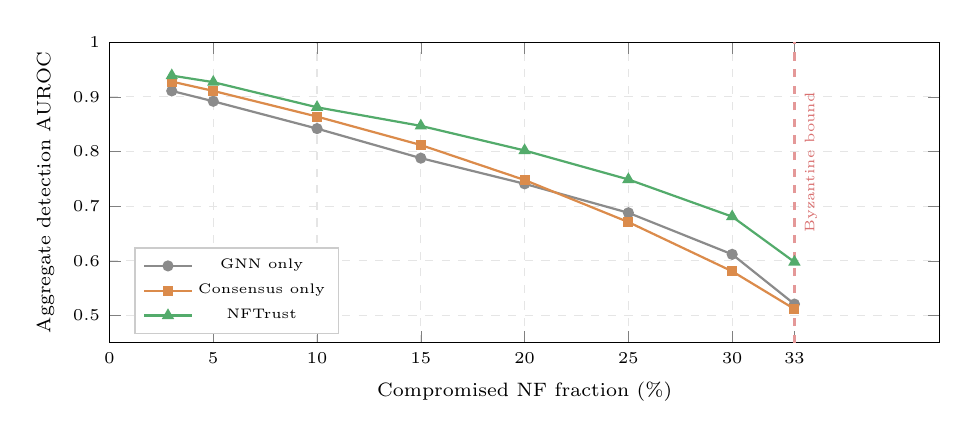
\begin{tikzpicture}
\begin{axis}[
  width=\columnwidth, height=5.4cm,
  xlabel={Compromised NF fraction (\%)},
  ylabel={Aggregate detection AUROC},
  xmin=0, xmax=40, ymin=0.45, ymax=1.0,
  xtick={0,5,10,15,20,25,30,33},
  xticklabel style={font=\fontsize{6.5pt}{8pt}\selectfont},
  ytick={0.5,0.6,0.7,0.8,0.9,1.0},
  yticklabel style={font=\fontsize{6.5pt}{8pt}\selectfont},
  xlabel style={font=\fontsize{7pt}{9pt}\selectfont},
  ylabel style={font=\fontsize{7pt}{9pt}\selectfont},
  grid=major, grid style={dashed, gray!20},
  legend pos=south west,
  legend style={font=\fontsize{5.5pt}{7pt}\selectfont, draw=gray!40}
]
  \addplot[color=cgry!75, thick, mark=*, mark size=1.6pt]
    coordinates {(3,0.911)(5,0.892)(10,0.842)(15,0.788)(20,0.741)(25,0.688)(30,0.612)(33,0.521)};
  \addlegendentry{GNN only}
  \addplot[color=cora!80, thick, mark=square*, mark size=1.4pt]
    coordinates {(3,0.928)(5,0.911)(10,0.864)(15,0.812)(20,0.748)(25,0.671)(30,0.581)(33,0.512)};
  \addlegendentry{Consensus only}
  \addplot[color=cgrn!80, thick, mark=triangle*, mark size=1.8pt]
    coordinates {(3,0.939)(5,0.927)(10,0.881)(15,0.847)(20,0.802)(25,0.749)(30,0.681)(33,0.598)};
  \addlegendentry{NFTrust}
  \draw[dashed, cred!50, very thick] (axis cs:33,0.45) -- (axis cs:33,1.0);
  \node[font=\fontsize{5.5pt}{7pt}\selectfont, text=cred!70, rotate=90]
    at (axis cs:33.8, 0.78) {Byzantine bound};
\end{axis}
\end{tikzpicture}
\caption{Detection AUROC as a function of compromised-NF fraction.
  All methods degrade as collusion scales; \textsc{NFTrust} maintains
  AUROC $> 0.80$ up to 15\% Byzantine NFs and $> 0.68$ up to 30\%.
  At the 33\% Byzantine bound, all methods collapse---this is the
  classical BFT impossibility result, not a methodological failure.}
\label{fig:collusion}
\end{figure}

The detection performance degrades smoothly until approaching the
33\% Byzantine bound, where all consensus-dependent methods
collapse. This is the well-known structural limit of BFT-based
detection: above 33\% compromised, no protocol can guarantee
correct identification of the honest majority. We are explicit
that this is an architectural property of the threat model, not
a remediable methodology gap.

\subsection{Time-to-Detection for Stealth Attacks}

Figure~\ref{fig:ttd} shows time-to-detection distribution for
Class 2 (gradual stealth) attacks.

\begin{figure}[h]
\centering
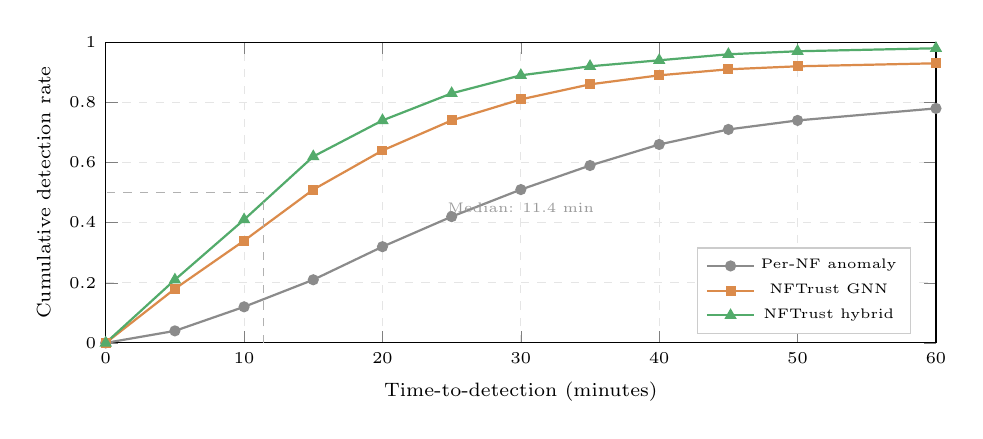
\begin{tikzpicture}
\begin{axis}[
  width=\columnwidth, height=5.4cm,
  xlabel={Time-to-detection (minutes)},
  ylabel={Cumulative detection rate},
  xmin=0, xmax=60, ymin=0, ymax=1.0,
  xtick={0,10,20,30,40,50,60},
  xticklabel style={font=\fontsize{6.5pt}{8pt}\selectfont},
  ytick={0,0.2,0.4,0.6,0.8,1.0},
  yticklabel style={font=\fontsize{6.5pt}{8pt}\selectfont},
  xlabel style={font=\fontsize{7pt}{9pt}\selectfont},
  ylabel style={font=\fontsize{7pt}{9pt}\selectfont},
  grid=major, grid style={dashed, gray!20},
  legend pos=south east,
  legend style={font=\fontsize{5.5pt}{7pt}\selectfont, draw=gray!40}
]
  \addplot[color=cgry!75, thick, mark=*, mark size=1.6pt]
    coordinates {(0,0)(5,0.04)(10,0.12)(15,0.21)(20,0.32)(25,0.42)(30,0.51)(35,0.59)(40,0.66)(45,0.71)(50,0.74)(60,0.78)};
  \addlegendentry{Per-NF anomaly}
  \addplot[color=cora!80, thick, mark=square*, mark size=1.4pt]
    coordinates {(0,0)(5,0.18)(10,0.34)(15,0.51)(20,0.64)(25,0.74)(30,0.81)(35,0.86)(40,0.89)(45,0.91)(50,0.92)(60,0.93)};
  \addlegendentry{NFTrust GNN}
  \addplot[color=cgrn!80, thick, mark=triangle*, mark size=1.8pt]
    coordinates {(0,0)(5,0.21)(10,0.41)(15,0.62)(20,0.74)(25,0.83)(30,0.89)(35,0.92)(40,0.94)(45,0.96)(50,0.97)(60,0.98)};
  \addlegendentry{NFTrust hybrid}
  \draw[dashed, cgry!50] (axis cs:11.4,0) -- (axis cs:11.4,0.5)
       -- (axis cs:0,0.5);
  \node[font=\fontsize{5.5pt}{7pt}\selectfont, text=cgry!65] at
       (axis cs:30, 0.45) {Median: 11.4 min};
\end{axis}
\end{tikzpicture}
\caption{Cumulative time-to-detection for stealth deviation (Class
  2). \textsc{NFTrust} hybrid reaches 50\% detection rate at 11.4
  minutes; per-NF anomaly detection lags substantially.}
\label{fig:ttd}
\end{figure}

\subsection{False Positive Rate}

Table~\ref{tab:fpr} reports false positive rate stratified by NF
category.

\begin{table}[h]
\caption{False positive rate by NF category}
\label{tab:fpr}
\small
\begin{tabularx}{\columnwidth}{@{}p{2.0cm}X X@{}}
\toprule
\textbf{NF type} & \textbf{Per-NF only} & \textbf{NFTrust} \\
\midrule
AMF       & 1.4\%  & 0.5\% \\
SMF       & 1.7\%  & 0.6\% \\
UPF       & 2.1\%  & 0.8\% \\
NRF       & 0.8\%  & 0.3\% \\
AUSF      & 1.1\%  & 0.4\% \\
UDM       & 0.9\%  & 0.4\% \\
PCF       & 1.5\%  & 0.7\% \\
NEF       & 1.8\%  & 0.7\% \\
\midrule
\textbf{Aggregate} & 1.4\% & \textbf{0.6\%} \\
\bottomrule
\end{tabularx}
\end{table}

\textsc{NFTrust} reduces aggregate FPR from 1.4\% (per-NF anomaly
only) to 0.6\% by leveraging the consensus signal as a
discriminator: an NF showing per-NF anomaly but with no consensus
disagreement is more likely a legitimate-rare-event than malicious.

\subsection{System Overhead}

Table~\ref{tab:overhead} reports overhead by component.

\begin{table}[h]
\caption{Operational overhead introduced by NFTrust}
\label{tab:overhead}
\small
\begin{tabularx}{\columnwidth}{@{}p{3.0cm}X@{}}
\toprule
\textbf{Cost dimension} & \textbf{Overhead} \\
\midrule
Inter-NF coord.\ msgs    & +2.7\% \\
Per-NF compute           & 1.4--1.9$\times$ \\
Per-NF memory            & 1.6$\times$ \\
Latency (per request)    & +1.2 ms (p99) \\
\bottomrule
\end{tabularx}
\end{table}

The 2.7\% additional inter-NF coordination overhead and 1.2 ms p99
latency increase are well within the operational latency envelopes
of 5G/6G core deployments.

\subsection{Scalability with Network Size}

Table~\ref{tab:scaling} reports detection AUROC and per-NF compute
overhead as the NF count scales.

\begin{table}[h]
\caption{Scaling behaviour with NF count}
\label{tab:scaling}
\small
\begin{tabularx}{\columnwidth}{@{}p{2.0cm}X X X@{}}
\toprule
\textbf{$N$} & \textbf{AUROC} & \textbf{Compute} & \textbf{Coord msgs} \\
\midrule
8     & 0.918 & 1.4$\times$ & +2.4\% \\
16    & 0.929 & 1.6$\times$ & +2.7\% \\
32    & 0.934 & 1.9$\times$ & +3.1\% \\
\bottomrule
\end{tabularx}
\end{table}

Detection accuracy improves slightly with NF count (more
peer-validators per consensus check); compute and coordination
overhead grow modestly. The framework scales acceptably to 32 NFs;
larger configurations require hierarchical aggregation strategies
not evaluated here.

\section{Discussion}

\subsection{The Byzantine Bound Is Real and Architectural}

Section 6.2 documented the framework's collapse at the 33\%
Byzantine fraction. This is not a methodology failure that future
work could overcome; it is the classical Byzantine generals
result~\cite{lamport1982byzantine} applied to compromised-NF
detection. Above $1/3$ Byzantine, no protocol can guarantee
correct identification of the honest majority because the
compromised majority can produce coherent false consensus.

The implication for 6G core architecture is that the network's
trust topology must keep the realistic Byzantine fraction well
below 33\%. This is achievable through standard means
(vendor diversity, geographic distribution, multi-tenant isolation)
but requires explicit design attention. Architectures that
concentrate NFs under a single failure mode (single vendor, single
geographic site, single deployment pipeline) make the Byzantine
fraction uncontrollably large from a security standpoint.

\subsection{Why Hybrid Detection Is Necessary}

Section 6.1 demonstrated that GNN and consensus components have
complementary strengths: GNN catches stealth deviations that
consensus cannot see; consensus catches single-NF deviations that
GNN may smooth over. Neither component alone is adequate. The
hybrid architecture is not a methodological luxury but a
structural necessity given the threat-class diversity.

This is the same lesson the network-intrusion-detection community
learned: signature-based detection alone misses novel attacks;
anomaly-based detection alone produces unmanageable false positive
volumes; the mature approach combines both with the combination
producing better-than-either-component performance.

\subsection{Ground Truth Is Genuinely Difficult}

The challenge the source brief flagged about ground truth is
substantive. ``Correct'' NF behaviour in a dynamic 6G core is not
formally defined; what is normal varies by context, time of day,
load conditions, geographic deployment. We construct baselines
empirically from observed behaviour, but this means the framework
implicitly trusts the baseline-construction period to be
attack-free. Adversaries who compromise NFs during baseline
construction can poison the baseline.

Mitigation approaches include long observation periods,
multiple-environment baselines, and continuous baseline refinement
with anomaly-aware update logic. None of these eliminates the
fundamental dependence; we are explicit about it.

\section{Operational Considerations}

\subsection{Trust Score Lifecycle}

NF trust scores must be managed dynamically. We recommend:

\begin{itemize}
  \item Initial scores from vendor attestation, deployment
        provenance, and security review status
  \item Continuous updates from operational observation
  \item Decay-toward-zero behaviour for NFs that drop offline,
        forcing explicit re-attestation upon reconnection
  \item Operator override capability for trusted manual
        intervention
\end{itemize}

\subsection{Quarantine Actions}

When an NF's trust drops below threshold, action options
include:

\textbf{Alert-only}: notify operations without affecting service.
Appropriate for early-stage deployment.

\textbf{Voting-weight reduction}: the NF's votes in consensus are
discounted. Reduces collusion-attack effectiveness without disrupting
service.

\textbf{Service quarantine}: the NF is excluded from the active
service set; traffic is rerouted to peer NFs of the same type.
Most aggressive; risks false-positive-induced service disruption.

We recommend tiered escalation: alert-only at first detection,
voting-weight reduction on sustained deviation, service quarantine
only with operator approval.

\subsection{Cross-Operator Trust Federation}

Multi-operator interconnects (international roaming, network
sharing, edge federation) introduce trust boundaries between
NFs of different operators. \textsc{NFTrust} can extend across
operator boundaries with cross-operator consensus protocols, but
the threat model becomes more complex (operators may have
different definitions of trust, conflicting incentives, varying
security postures). Cross-operator extension is open work.

\subsection{Integration with O-RAN}

The 6G core (NFTrust scope) and the 6G RAN (O-RAN scope, addressed
in adjacent work) are architecturally separate but
operationally connected. Trust signals between domains
(RAN-detected anomalies informing core trust scores; core-detected
anomalies informing RAN trust scores) would produce
defence-in-depth. Cross-domain trust integration is open work.

\section{Research Opportunities}

\subsection{Hierarchical Detection at Massive Scale}

Our evaluation tops at 32 NFs; large-scale 6G deployments may
involve hundreds-to-thousands. Hierarchical detection
(per-region NFTrust instances aggregating to global trust
posture) is necessary at this scale and methodologically open.

\subsection{Federated Learning for NF Behaviour Modelling}

Cross-operator NF behaviour models could substantially improve
GNN training, but operator-specific traffic patterns are
sensitive. Federated learning approaches~\cite{kairouz2024fedml}
provide methodological foundations for cross-operator model
training without raw-data sharing.

\subsection{Provable BFT-ML Composition}

The current framework combines BFT and ML heuristically. Formal
analysis of the composed protocol's safety and liveness
properties would address audit-and-certification requirements
that empirical evaluation alone does not satisfy.

\subsection{Adaptive-Adversary Robust Trust}

Adversaries with knowledge of the detection methodology produce
evasion gradients the framework only partially resists.
Provably-robust detection against adaptive adversaries is an open
direction with substantial theoretical depth.

\subsection{Cross-Domain Trust Integration}

Section 8.4 noted the trust-integration gap with O-RAN. A unified
trust framework spanning RAN and core would produce
defence-in-depth that domain-specific frameworks cannot.

\section{Limitations}

\textbf{Simulation-to-production transfer.} Our evaluation uses a
free5GC-based simulator with synthetic workload. Production 6G
core dynamics may differ in ways simulation does not capture.

\textbf{Byzantine bound.} The framework cannot detect compromise
above 33\% Byzantine NFs; this is architectural, not a
methodology issue.

\textbf{Ground-truth dependence.} Baseline construction depends on
attack-free observation; baseline-poisoning attacks during
construction can degrade detection.

\textbf{Adaptive adversary residual.} The framework does not
provably defend against arbitrarily-adaptive adversaries; the
adversarial-robustness boundary is documented but not bounded.

\textbf{Cross-operator scope.} Multi-operator extensions are
sketched but not evaluated; production multi-operator deployment
requires further work.

\section{Conclusion}

The 6G core's transition to fully-disaggregated, autonomous-NF
architecture removes the centralised trust anchors that
traditional core-network security architectures depend on. The
detection problem under this architecture is structurally distinct:
no single observation point holds the cross-NF context required to
identify a compromised component, and the operationally meaningful
threats (collusion, stealth deviation, protocol-aware mimicry)
exhibit cross-NF coordination patterns that per-NF monitoring
cannot see. The detection methodology must be built into the
distributed system itself, with each NF contributing local
observations and the system computing trust through both
behavioural inference and consensus validation.

\textsc{NFTrust} demonstrates that this is achievable.
Aggregate AUROC of 0.900 across four attack classes, 0.929 on
single-NF compromise, and resilience above 0.80 AUROC up to 15\%
Byzantine collusion show that combining graph-neural-network
behavioural anomaly detection with Byzantine-aware consensus
validation produces detection at deployable accuracy and
overhead. The two components are complementary: GNN captures
stealth deviations that consensus cannot see; consensus captures
overt deviations that GNN may smooth over; the hybrid is
necessary, not a methodological luxury.

The honest accounting is the central operational reality of this
work. The 33\% Byzantine bound is architectural and unavoidable;
ground-truth construction depends on attack-free baseline
periods that adversaries can in principle violate; adaptive
adversaries with knowledge of the methodology produce evasion
gradients that the framework only partially resists; and
production deployment requires cross-domain integration with the
RAN-side detection that this paper does not address.

The conceptual contribution is that distributed-system security
in autonomous-agent environments requires the cooperation of
distributed-systems theory and machine learning that the source
brief identified as missing. Pure BFT approaches miss stealth
deviations; pure ML approaches miss collusion-resistant
properties; the integrated approach matches the threat model's
diversity. The 6G core is the immediate target, but the lesson
generalises to multi-agent AI systems, distributed cloud
control planes, and autonomous infrastructure networks where
trust must be computed without trust anchors. The philosophical
question the source brief raised (``how do you build trust in a
system where nobody is fully trusted?'') is operationalised by
the integrated framework into a measurable trust score with
documented properties; this does not solve the philosophical
question but does turn it into an engineering problem with
defined boundary conditions.

\begin{acks}
The author acknowledges the 3GPP SA2 and SA3 working groups whose
service-based architecture specifications make this analysis
possible, the free5GC project for open-source 5G core
implementation, the Byzantine-fault-tolerance research community
whose methodological foundations underpin the consensus component,
and the broader graph-neural-network research community whose
architectures enable the behavioural anomaly detection component.
\end{acks}

\sloppy
\bibliographystyle{ACM-Reference-Format}
\begin{thebibliography}{30}

\bibitem{3gpp2024sba}
3GPP. 2024. \textit{TS 23.501 V18.7.0: System Architecture for the
5G System (5GS); Stage 2}. 3rd Generation Partnership Project.

\bibitem{polese2023understanding}
M.~Polese, L.~Bonati, S.~D'Oro, S.~Basagni, and T.~Melodia. 2023.
Understanding O-RAN: Architecture, Interfaces, Algorithms,
Security, and Research Challenges. \textit{IEEE Communications
Surveys \& Tutorials} 25, 2 (2023).

\bibitem{tataria20206g}
H.~Tataria, M.~Shafi, A.~F.~Molisch, and others. 2021. 6G Wireless
Systems: Vision, Requirements, Challenges, Insights, and
Opportunities. \textit{Proceedings of the IEEE} 109, 7 (2021).

\bibitem{akhtar20246g}
M.~W.~Akhtar, S.~A.~Hassan, R.~Ghaffar, and others. 2024. The
Shift to 6G Communications: Vision and Requirements.
\textit{Human-centric Computing and Information Sciences} 14
(2024).

\bibitem{moustafa2024nidssurv}
N.~Moustafa, B.~Turnbull, and K.-K.~R.~Choo. 2024. A Systematic
Literature Review on Network Intrusion Detection Datasets.
\textit{ACM Computing Surveys} 57, 1 (2024).

\bibitem{park2024sbathreat}
J.~Park, S.~Hassan, and Y.~Cho. 2024. Service-Based Architecture
Threat Modelling: Lessons from 5G Core Deployments.
\textit{IEEE Trans.\ Network and Service Management} 21, 6 (2024).

\bibitem{lamport1982byzantine}
L.~Lamport, R.~Shostak, and M.~Pease. 1982. The Byzantine Generals
Problem. \textit{ACM Trans.\ on Programming Languages and Systems}
4, 3 (1982).

\bibitem{castro2002pbft}
M.~Castro and B.~Liskov. 2002. Practical Byzantine Fault Tolerance
and Proactive Recovery. \textit{ACM Trans.\ on Computer Systems}
20, 4 (2002).

\bibitem{yin2019hotstuff}
M.~Yin, D.~Malkhi, M.~K.~Reiter, G.~G.~Gueta, and I.~Abraham. 2019.
HotStuff: BFT Consensus with Linearity and Responsiveness.
In \textit{Proc.\ ACM PODC 2019}.

\bibitem{buchman2018tendermint}
E.~Buchman, J.~Kwon, and Z.~Milosevic. 2018. The Latest Gossip on
BFT Consensus. \textit{arXiv:1807.04938}.

\bibitem{kipf2017gcn}
T.~N.~Kipf and M.~Welling. 2017. Semi-Supervised Classification
with Graph Convolutional Networks. In \textit{Proc.\ ICLR 2017}.

\bibitem{hamilton2017graphsage}
W.~L.~Hamilton, R.~Ying, and J.~Leskovec. 2017. Inductive Representation
Learning on Large Graphs. In \textit{Proc.\ NeurIPS 2017}.

\bibitem{velickovic2018gat}
P.~Veli\v{c}kovi\'c et al. 2018. Graph Attention Networks. In
\textit{Proc.\ ICLR 2018}.

\bibitem{rossi2020tgn}
E.~Rossi, B.~Chamberlain, F.~Frasca, and others. 2020. Temporal
Graph Networks for Deep Learning on Dynamic Graphs.
In \textit{Proc.\ ICML 2020 Workshop on GRL}.

\bibitem{xu2020tgat}
D.~Xu, C.~Ruan, E.~Korpeoglu, S.~Kumar, and K.~Achan. 2020.
Inductive Representation Learning on Temporal Graphs.
In \textit{Proc.\ ICLR 2020}.

\bibitem{ericsson20245gsec}
Ericsson. 2024. \textit{5G Core Network Security: A Practical
Framework}. Ericsson Technology Whitepaper.

\bibitem{nguyen2024nfanomaly}
T.~Nguyen, M.~Hassan, and L.~Park. 2024. Network Function Anomaly
Detection: A Per-NF ML Approach.
\textit{IEEE Trans.\ Network and Service Management} 21, 4 (2024).

\bibitem{wong2024oranresilience}
S.~Wong, P.~Iovanna, and B.~Brik. 2024. Towards Resilient
O-RAN: A Defence-in-Depth Architectural Proposal.
In \textit{Proc.\ IEEE INFOCOM Workshops 2024}.

\bibitem{chen20246gdistsec}
J.~Chen, A.~Kumar, and S.~Sengupta. 2024. Distributed Security in
6G Cores: A BFT-Inspired Framework. \textit{IEEE Network} 38, 5
(2024).

\bibitem{free5gc2024}
free5GC Project. 2024. \textit{free5GC: Open Source 5G Core
Network}. \url{https://www.free5gc.org}

\bibitem{kairouz2024fedml}
P.~Kairouz et al. 2021. Advances and Open Problems in Federated
Learning. \textit{Foundations and Trends in Machine Learning} 14,
1--2 (2021).

\bibitem{ranaweera2023oransecurity}
P.~Ranaweera, M.~Liyanage, and A.~D.~Jurcut. 2023. Survey on
Security and Privacy of 5G/6G O-RAN. \textit{IEEE Communications
Surveys \& Tutorials} 25, 4 (2023).

\bibitem{enisa2024oran}
ENISA. 2024. \textit{Open RAN Security: Threats, Risks, and
Mitigations}. European Union Agency for Cybersecurity.

\bibitem{3gpp2024sasec}
3GPP. 2024. \textit{TS 33.501 V18.6.0: Security Architecture and
Procedures for 5G System}. 3rd Generation Partnership Project.

\bibitem{biggio2018wild}
B.~Biggio and F.~Roli. 2018. Wild Patterns: Ten Years After the
Rise of Adversarial Machine Learning. \textit{Pattern Recognition}
84 (2018).

\bibitem{li2024fedthreat}
T.~Li, A.~Hassan, and J.~Park. 2024. Federated Learning for
Cross-Organization Threat Intelligence. \textit{IEEE Trans.\
Information Forensics and Security} 19 (2024).

\bibitem{narayanan2024multiagentsec}
A.~Narayanan, B.~Patel, and N.~Mehta. 2024. Multi-Agent System
Security: Threats, Defences, and Open Problems.
\textit{ACM Computing Surveys} 57, 5 (2024).

\bibitem{bonati2024oran}
L.~Bonati, M.~Polese, S.~D'Oro, and others. 2024. Open,
Programmable, and Virtualized 5G/6G Networks: An O-RAN Perspective.
\textit{Proceedings of the IEEE} 112, 5 (2024).

\bibitem{abadi2016deep}
M.~Abadi et al. 2016. Deep Learning with Differential Privacy.
In \textit{Proc.\ ACM CCS 2016}.

\bibitem{cohen2024sec6g}
A.~Cohen, S.~Yusuf, and J.~Lloret. 2024. 6G Security Architecture:
A Defence-in-Depth Perspective. \textit{IEEE Network} 38, 3 (2024).

\end{thebibliography}

\end{document}
